% \section{\shibato{コード断片追跡アルゴリズムの改良}{}}


\section{コード断片追跡アルゴリズムの改良}

\label{section:Piece_level_Diff_Backtrack_Algorithm}

\subsection{LHDiffの改良方法}
CodeGlassのサーバは,ユーザが選択したコード断片に関連する過去のコミットを抽出する必要がある.
gitのコマンドであるblameを使う事で,コード断片を最後に変更したコミットを特定する事ができる.
しかし,gitのコマンドではコード断片が過去のバージョンにおけるソースコードのどこに存在するのかを知る事ができない.
したがって,ユーザが選択したコード断片に関連する過去のコミットを最新のものだけでなく全て抽出するためには,選択されたコード断片が過去のバージョンにおいてどこに存在するのかを特定する必要がある.
%以上の手法を実装するために,我々はサーバ上のアルゴリズムについて次の3つの要件を設けた.


% The CodeGlass server system needs to obtain commits that involve changes on the code piece selected by the user.
% Such an algorithm needs to locate the portion in a past commit which best matches with the given code piece.
% To make CodeGlass viable in realistic use, we have the following design considerations for the algorithm.

%       \begin{figure}[!t]
%         \centering
%             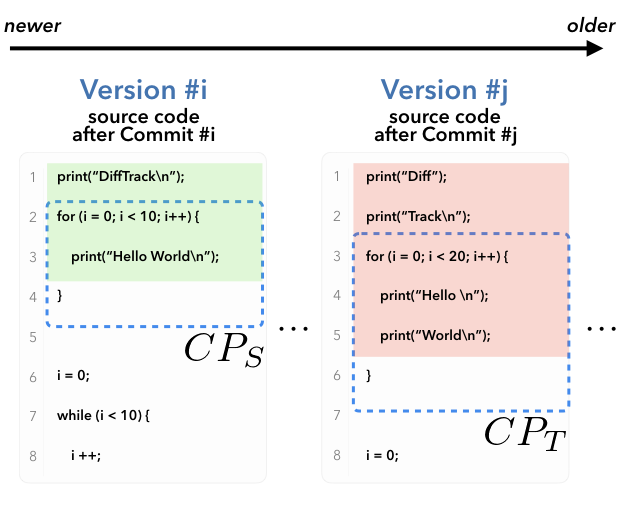
\includegraphics[width=0.9\columnwidth]{algorithm/limitation.png}
%             \caption{An example illustration of a source and true target code piece ($CP_{S}$ and $CP_{T}$). In this and following figures, red and green lines represent deleted and added lines between two versions (\#$i$ and \#$j$, $i>j$), respectively. A code piece in the newer version serves as $CP_S$ (lines in the broken frame in Version \#i). A backtrack algorithm estimates the location of $CP_{T}$ given $CP_{S}$, and runs iteratively with older commits. An estimated target code piece is denoted as $\widehat{CP_{T}}$. The ideal $\widehat{CP_{T}}$ is $CP_{T}$. This backtracking returns a series of commits associated with the code piece originally selected by the user.}

% \label{fig:CommitHistory}
%       \end{figure}

% \begin{itemize}
% \setlength{\parskip}{1mm}
% \setlength{\leftskip}{4mm}
% \setlength{\itemsep}{0cm}
% \item[DC-1.] 選択されたコード断片が過去のバージョンに含まれる場合,その位置を正確に特定する事.
% %\item[DC-2.] Run in real time regardless of the project scale and code length as well as the size of a code piece.
% \item[DC-2.] プログラミング言語(スタイルシートや設定ファイルを含む)に依存する事なく動作する事.
% \item[DC-3.] コードの行単位の粒度で動作する事.
% \end{itemize}

% \begin{itemize}
% \setlength{\parskip}{1mm}
% \setlength{\leftskip}{4mm}
% \setlength{\itemsep}{0cm}
% \item[DC-1.] Accurately identify the location of a code piece in an older version even if changes occurred within it.
% %\item[DC-2.] Run in real time regardless of the project scale and code length as well as the size of a code piece.
% \item[DC-2.] Be compatible with any type of program-related files including style sheets and configuration files.
% \item[DC-3.] Perform at a line-level granularity to support unconstrained interaction.
% \end{itemize}

% \shibato{}{source code piece を被選択コード断片,target code piece を目的コード断片と翻訳しました}

アルゴリズムを説明するために,まず被選択コード断片と目的コード断片を定義する.
被選択コード断片($CP_{S}$)は,ユーザがCodeGlassのインターフェース上で選択したコード断片である.
また目的コード断片は,過去のバージョンにおける被選択コード断片と対応したコード断片である.
アルゴリズムは$CP_{S}$の情報を受け取り,過去のバージョン内の目的コード断片の位置を推定する.
ここで,正解目的コード断片($CP_{T}$)と推定目的コード断片($\widehat{CP_{T}}$)を新たに定義する.
正解目的コード断片は過去のバージョンにおける$CP_{S}$にマッチするコード断片である.
また,推定目的コード断片はアルゴリズムが推定した過去のバージョンにおける被選択コード断片を意味する.
アルゴリズムが完全に正しく動作した場合,$\widehat{CP_{T}}$と$CP_{T}$が一致する.
% \shibato{
% また,アルゴリズムは過去のバージョン数に合わせて繰り返し実行されるため,$i$をコード断片のバージョンの順番番号と定義する.
% 即ち,$CP_{Ti}$は最新から$i$番目のバージョンにおける正解目的コード断片である.
% }{ここ使ってないので消してもいいかも}

% To explain the details of the algorithm, we first define a source and target code piece.
% A source code piece ($CP_{S}$) is a code piece in a commit.
% Using $CP_{S}$, our algorithm estimates a target code piece in an older commit.
% We denote a true and estimated target code piece as $CP_{T}$ and $\widehat{CP_{T}}$, respectively.
% Ideally, $\widehat{CP_{T}}$ is exactly the same set of lines of $CP_{T}$.
% As our algorithm is executed iteratively, an additional subscript $i$ represents a code piece in the $i$-th version from the initial commit (i.e., $CP_{Si}$ is the source code piece in Version \#$i$).
%We assume that the number of $CP_T$ is always one.

%The iteration occurs by using a target code piece as the source in the next step (i.e., $CP_{Sj} = \widehat{CP_{Ti}}$, $i>j \geq 1$).

% \subsection{Limitations with git and git-blame commands}
% \label{subsection:Limitations_with_git_commands}


%     \begin{figure}[tb]
%             \centering
%           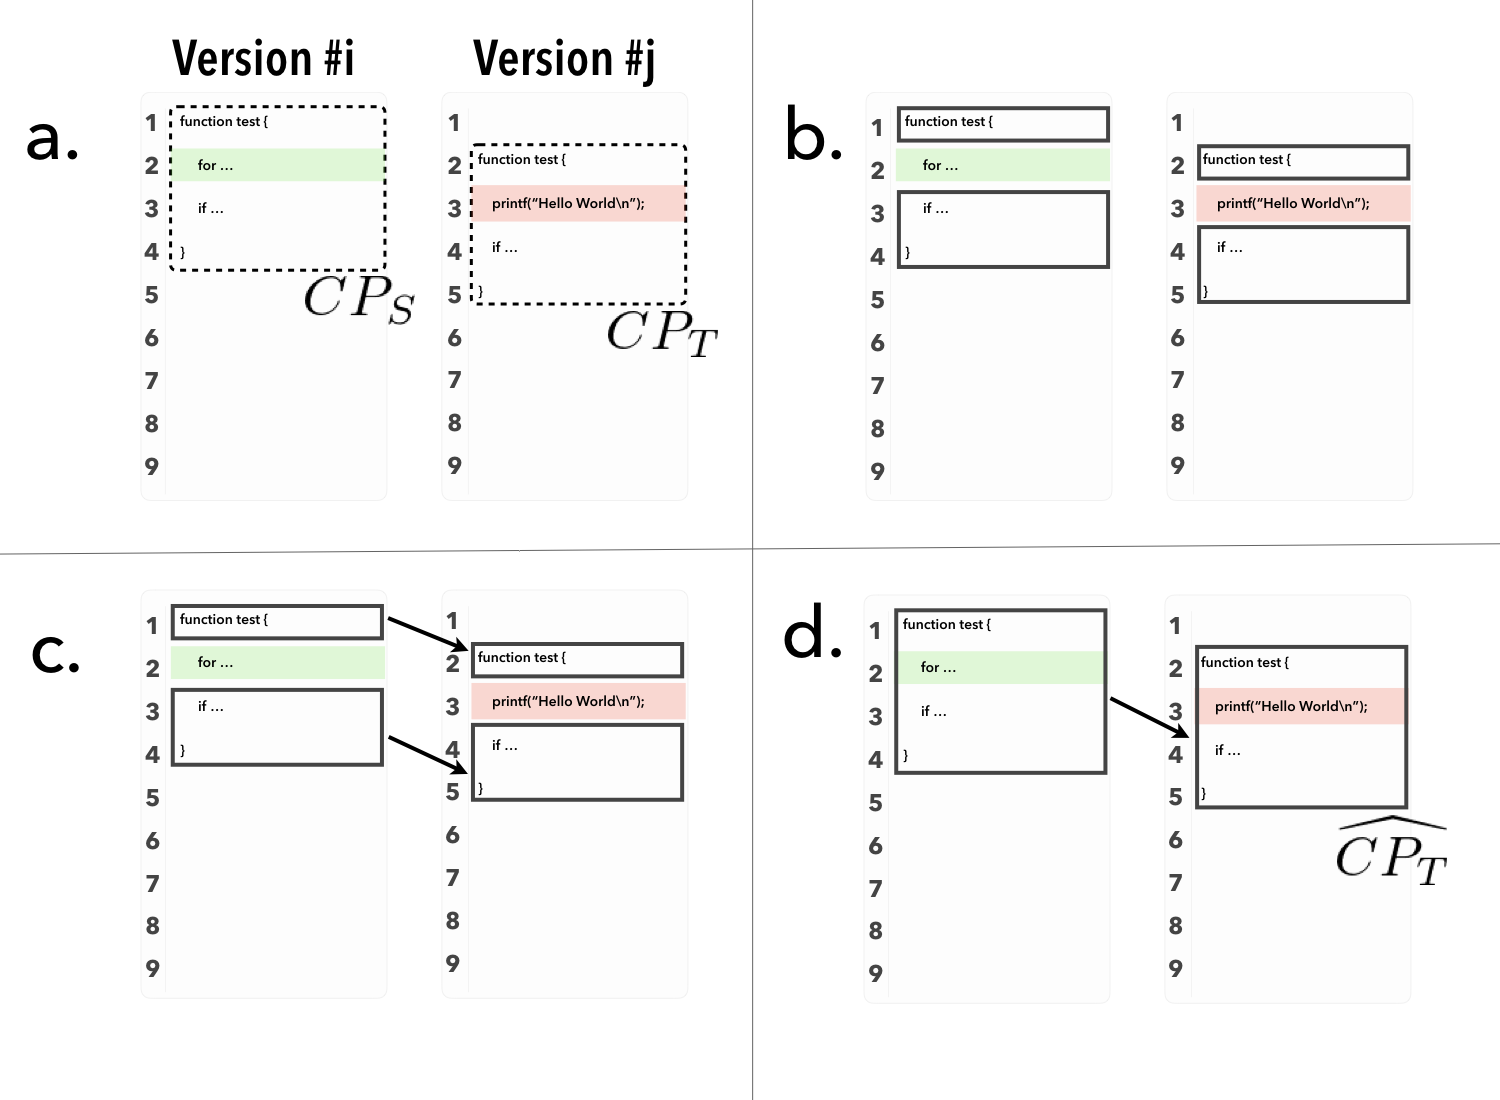
\includegraphics[width=1.0\columnwidth]{algorithm/Cases_001.png}
%           \caption{Case A: $CP_S$ includes unchanged lines that enclose the revised portion. (a) $CP_S$ and $CP_T$ are line 1--4 in the source commit and line 2--5 in the target commit, respectively. (b) The unchanged lines in $CP_S$ enclose the revised portion. (c) The unchanged lines serve as an anchor for search. (d) DiffTrack thus immediately determines line 2--5 as $\widehat{CP_T}$.}
%           \label{fig:caseA}
%     \vspace{-2mm}
%     \end{figure}


%     \begin{figure}
%       \centering
%         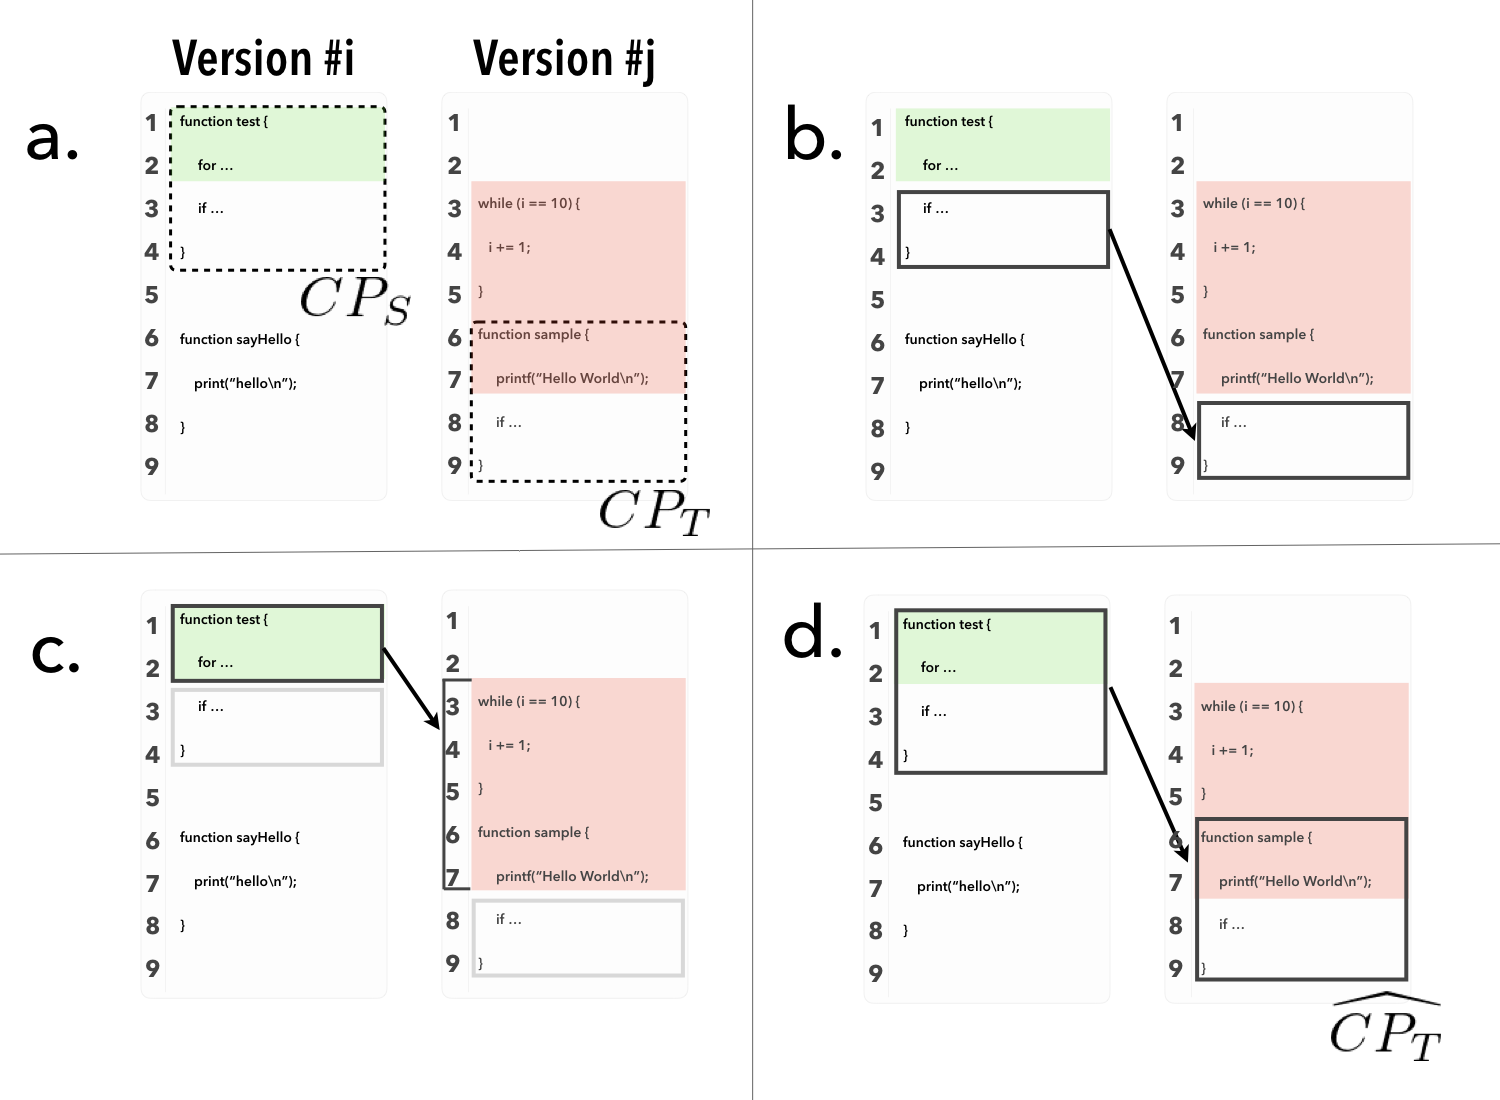
\includegraphics[width=1.0\columnwidth]{algorithm/Cases_002.png}
%         \caption{Case B: $CP_S$ includes unchanged lines that do not enclose the revised portion. (a) $CP_S$ and $CP_T$ are line 1--4 in the source commit and line 6--9 in the target commit, respectively. (b) DiffTrack first performs matching with the unchanged lines. (c) It removes unchanged lines (line 1 and 2) in the target commit from the search space. (d) It then performs fuzzy string search matching to identify lines most similar to the revised lines in the source commit. It finally determines line 6--9 $\widehat{CP_T}$.}~\label{fig:caseB}
%     \vspace{-5mm}
%     \end{figure}


% Figure~\ref{fig:CommitHistory} shows an example of code changes between two versions (\#$i$ and \#$j$, $i > j$).
% Suppose that our system needs to identify commits related to line 2--4 in Version \#$i$ to extract associated pull requests.
% Thus, this portion is $CP_{Si}$~(the broken frame in Version \#$i$ in Figure~\ref{fig:CommitHistory}).
% The git-blame command can point to the latest commit in which any part of $CP_{Si}$ was affected.
% Thus, it is straightforward to find Commit \#$j$.
% However, it provides \textit{only} the latest commit that contains changes in $CP_{Si}$.
% This means that a system needs to find $CP_{Sj}$ (or $CP_{Ti}$) given $CP_{Si}$ to trace back to older commits and iteratively perform git-blame.
% However, a diff log merely contains a set of line additions and deletions, which do not directly represent which revised lines are related to $CP_{Si}$.
% In other words, git-blame cannot immediately provide the location of $CP_{Ti}$.
% In the example of Figure~\ref{fig:CommitHistory}, a system can only know that there are three lines of additions and five lines of deletions.
% But it is not immediately clear which revised lines are related to $CP_{Si}$, and we thus need a method to estimate the location of $CP_{Ti}$ (which also serves as $CP_{Sj}$ for further backtracking).

% \subsection{Limitations with abstract syntax trees}

% Another alternative approach is to use fine-grained source code change extraction methods~\cite{GumTree, Change_Distilling}.
% These approaches can extract not only additions or deletions but also infer syntactic changes, such as updates or moves.
% They use an abstract syntax tree (AST) to compute similarity between the two versions and extract syntactic changes.
% %One example of such algorithms is Change Distiller developed by Fluri et al~\cite{Change_Distilling}.
% %Falleri et al.'s GumTree~\cite{GumTree} further improve precisions on detecting code moves.
% Although these algorithms are designed to compare multiple versions of an entire source code file, it is theoretically possible to implement them to perform matching of code pieces.


% Nevertheless, we decided not to consider AST-based methods because they do not satisfy DC-2 and 3 in general.
% As methods using abstract syntax trees require a parser, additional configuration is necessary for adaptation to different programming languages.
% For example, GumTree~\cite{GumTree} is only compatible with C, Java, JavaScript, and Ruby as of April 2017.
% Internal parsing can lead to large computational overhead for long code pieces.
% In addition, a selected code piece should be syntactically correct, which also limits user experience.
% We thus developed an algorithm called DiffTrack.

% \koji{}{If we have anything besides LHDiff to be discussed, add it here and explain why we don't use it.}

先行研究では,コード断片を過去のバージョンの中で追跡する手法が提案されており,それらをCodeGlassのサーバのアルゴリズムとして活用できる可能性がある.
% 例えばSpaccoとWilliams~\cite{SDiff}が実装したSDiffというアルゴリズムは,抽象構文木を用いてコードを解析する事で,コード断片を過去のバージョンの中で追跡する事ができる.
% しかし,SDiffが動作するためには構文解析を行う必要があるため,DC-2を満たす事が出来ない.
Asaduzzamanら~\cite{LHDiff}が開発したLHDiffは,プログラミング言語非依存で動作するコード断片追跡アルゴリズムである.
LHDiffはword-level fuzzy matching~\cite{sankoff1983time}を用いて$CP_{S}$と$\widehat{CP_T}$との文字列的類似度を計算し,最も類似度が高かったものを$CP_{T}$として決定する.
%LHDiffは要件DC-2とDC-3を満たしており,かつ評価実験ではその他のコード断片追跡アルゴリズムよりも正確であった事から,要件DC-1も満たしている.

% 過去のバージョン内でコード断片を追跡するアルゴリズムに関する先行研究が複数存在する.
% SpaccoとWilliams~\cite{SDiff}が実装したSDiffというアルゴリズムは,抽象構文木を用いてコード断片を追跡する事ができる.
% SDiffが動作するためには構文解析を行う必要があるため,プログラミング言語に依存する.
% 一方でAsaduzzamanら~\cite{LHDiff}が開発したLHDiffは,プログラミング言語非依存で動作するコード断片追跡アルゴリズムである.
% LHDiffは\shibato{fuzzy string matching}{日本語にする必要ある?}を使用しコード断片と$\widehat{CP_T}$の候補との文字列的類似度をそれぞれ計算する事で,$\widehat{CP_T}$を推定する.
% そして最も類似度が高かったコード断片を$\widehat{CP_T}$として決定する.
% LHDiffは要件DC-2とDC-3満たしており,かつAsaduzzamanらによる評価実験ではその他のコード断片追跡アルゴリズムよりも正確であった事から,要件DC-1も満たしている.

% There exist different algorithms for backtracking code changes across revisions.
% SDiff developed by Spacco and Williams~\cite{SDiff} uses abstract syntac trees for backtracking.
% This algorithm requires syntactic analysis, and thus it is language-dependent.
% In contrast to SDiff, Asaduzzaman et al. demonstrated a language-agnostic algorithm, called LHDiff~\cite{LHDiff}.
% It uses fuzzy string matching and calculates similarity between the given code piece and candidates of $\widehat{CP_T}$.
% LHDiff then determines $\widehat{CP_T}$ as a code piece with the highest similarity score.
% This algorithm satisfies DC-2 and DC-3.
% In addition, their evaluation showed that LHDiff achieves a high accuracy performance compared to other code tracking techniques and thus meets DC-1.

しかし我々がLHDiffの事前調査を行った結果,コード変更が構造的変更(関数の統合や分裂,リファクタリングなど)を含む場合,LHDiffはコード断片の追跡に失敗する事が分かった.
この原因は,LHDiffでは$CP_T$が一つしか存在しないと仮定されているからである.
実際のコード変更履歴では,被選択コード断片が過去のバージョンにおいて他のコード断片と統合されていたり,分割されて実装されていたりする可能性がある.
特に大規模なソフトウェア開発プロジェクトでは,ソースコードの構造的変更が繰り返し行われる事が多いため,LHDiffをそのままCodeGlassのサーバに実装すると,CodeGlassの実用性が制限されてしまう.
そこで我々は,LHDiffに新たにgraceful matchingを導入することでこの問題を解決することを試みた.

% However, our pilot study on the na\"{i}ve LHDiff method found that it fails to backtrack when revisions involve structural changes (e.g., merge and refactoring) because it assumes that the number of $CP_T$ is always one.
% This may cause degradation of the utility of CodeGlass.
% To address this issue, we integrated a graceful code matching mechanism into LHDiff.


LHDiffは$CP_T$が常に一つであるという仮説の下,最も文字列的類似度が高いコード断片を$\widehat{CP_T}$として決定する.
我々は新たに,正解目的コード断片が一つに定まる可能性が高い事を示す閾値であるDMT(Definitive Matching Threshold)を導入した.
$CP_{S}$と$\widehat{CP_T}$の候補の文字列的類似度がDMTよりも高かった場合,LHDiffと同様に$\widehat{CP_T}$を決定する.
しかし,過去にソースコードの構造的な変更や大規模な修正が行われていると,文字列的類似度が低くなり,$CP_{T}$を正確に一意に推測する事が難しくなる.
そこで,別の閾値であるCMT(Candidate Matching Threshold)を導入する.
DMTを上回る$\widehat{CP_T}$が存在しなかった場合,CMTを上回るコード断片を全て,$CP_{T}$である可能性があるとしてインターフェースに返す.
CodeGlassのインターフェースは,それらのコード断片を含むコミットを図~\ref{fig:WebInterface}a~(3)のように表示する.
ユーザはそのコミットをクリックして過去のバージョンにおけるソースコードを確認し,$CP_S$として選択し直す事で,引き続きコード断片の調査を継続する事ができる.
% ユーザはそのコミットをクリックして過去のバージョンにおけるソースコードを確認し,\sakaguchi{$CP_{T}$を特定してから}{ユーザが正解目的コード断片を特定するというのに違和感を覚えます…CPtはあくまで学習におけるシンボルな気がします}それを$CP_S$として選択し直す事で,引き続きコード断片の調査を継続する事ができる.

% The na\"{i}ve LHDiff method determines $\widehat{CP_T}$ as a code piece with the highest similarity under an assumption that the number of $CP_T$ is always one.
% We introduce a threshold (Definitive Matching Threshold, DMT) to determine if there exists a single possible target code piece with strong belief.
% But the fuzzy string matching method may still fail to find a single $\widehat{CP_T}$ when changes are substantial.
% To allow graceful matching, we introduce another threshold (Candidate Matching Threshold, CMT).
% The graceful matching creates a list of likely target code pieces instead of simply stopping search.


DMTとCMTの二つの閾値を設定するために,Chart.jsのリポジトリに含まれる49個のコミットにおける,変更前と変更後のコード断片の一対をデータセットとして構築した.
このデータセットではLHDiffだけでは$CP_{T}$を特定する事が難しい構造的変更からなるコミットのみを意図的に選定した.
そして,それぞれのコード断片に対して$CP_S$を選択し,それに対応する$CP_T$のラベル付けを行った.
% そして,それぞれのコード断片に対して\sakaguchi{$CP_S$}{そういえば学習におけるCPsはどう決めるんでしょう?}と$CP_T$のラベル付けを行った.
さらに,$CP_T$と最も文字列的類似度の高い,$CP_T$ではないコード断片を$IM$(incorrect match)としてラベル付けした.
% \sakaguchi{}{目的コード断片の定義がちゃんとわかっていないのですが単純に似たコードということでしょうか…?ちなみに同じ内容の断片が複数ファイルに合った場合どうなるでしょう…?}


% To determine appropriate values for these threshold, we created a dataset containing 49 commits (i.e., 49 pairs of two versions) in Chart.js.
% This dataset deliberately contained only refactoring revisions.
% Estimating a match in these revisions is presumably difficult with the na\"{i}ve LHdiff algorithm.
% In each pair, we manually labeled $CP_S$ and $CP_T$.
% We also chose a code piece which was a disjoint set of $CP_T$ and exhibited the highest similarity as the most similar incorrect match ($IM$).

図~\ref{fig:histogram_sim}に$CP_T$(青)と$IM$(橙)の文字列的類似度の分布を示す.
この分布から$IM$の類似度は0.65未満である事が分かる.
また,$CP_T$の類似度は0.4より大きい事も分かる.
したがって我々は,DMTを0.65に,CMTを0.4に設定した.

% Figure~\ref{fig:histogram_sim} shows the distributions of similarity scores of $CP_T$ (in blue) and $IM$ (in pale orange).
% This histogram clearly illustrates that similarity scores of $IM$ are below 0.65.
% It also shows that the scores of $CP_T$ are above 0.45.
% We, therefore, determined DMT and CMT to be 0.65 and 0.4, respectively.


% 我々のコード断片追跡アルゴリズムは,ユーザが選択したコード断片内でのコード変更を含むコミットの一覧を特定する.
% アルゴリズムはまず最初に,git-blameを用いてコード断片の最新のコミットを特定する.
% 次にLHDiffにより最も文字列的類似度の高いコード断片を$\widehat{CP_T}$として決定する.
% この処理を繰り返し行い,DMTを上回るコード断片が見つからなかった時に動作を終了する.

% Our tracking algorithm can identify a set of commits that contain changes on a user-selected code piece.
% It first finds the latest commit containing changes on the code piece by the git-blame command.
% LHDiff then locates a portion of code in this version which is the most similar to the given code piece (i.e., $\widehat{CP_T}$).
% It then performs this operation iteratively by using the estimated portion of code as the next source code piece to trace back to even older versions.
% Our algorithm stops backtracking when it finds no code piece with a higher value than DMT.

% \shibato{graceful matching}{}は,追加でCMTを上回る正解目的コード断片の可能性があるコード断片を探索する.
% コード断片がコミットにおいて別ファイルへ移動した可能性も考慮して,\shibato{graceful matching}{}は変更のあった全てのファイルを探索する.
% そして見つかった正解目的コード断片の可能性があるコード断片を文字列的類似度順に並び替える.
% 次にそれらのコード断片が互いに排他的である事を確認してから,インターフェースに返す.
% インターフェース上では正解目的コード断片の可能性があるコード断片はFigure~\ref{fig:WebInterface}a(2)のように示される.

% With graceful matching, the algorithm additionally searches all possible code pieces with the similarity scores above CMT after backtracking.
% In order to capture cases in which a code piece was moved from a file to another, the graceful matching process checks all revised files in the repository. 
% The algorithm first sorts possible target code pieces by their similarity scores in the descending order, and initializes a list for candidate target code pieces.
% For each possible code piece, the algorithm checks if it is mutually exclusive with all lines in the current candidate list.
% If true, the algorithm adds that code piece to the candidate list.
% All code pieces in this candidate list are finally shown to the user in the interface ((2) in Figure~\ref{fig:WebInterface}a).


% \subsubsection{Case A: $CP_S$ includes unchanged lines that enclose the revised portion.}


% $CP_S$ contains revised lines between the unchanged portions (i.e., line 2 in Version \#i in Figure~\ref{fig:caseA}).
% In this case, the algorithm first uses the unchanged lines (line 1, 3, and 4) as an anchor to find $\widehat{CP_T}$.
% In addition, only changed lines should be included between the unchanged portions.
% The algorithm, therefore, immediately identifies $\widehat{CP_T}$ as the unchanged portions and changed lines in-between (i.e., line 2--5 in Version \#$j$).

% \subsubsection{Case B: $CP_S$ includes unchanged lines that do not enclose the revised portion.}

%     \begin{figure}[tbp]
%             \centering
%           \includegraphics[clip, width=8cm]{algorithm/CaseB.png}
%           \caption{An example of case B (where $CP_S$ includes unchanged lines that do not enclose the revised portion).
%           $CP_S$ and $CP_T$ are from line 1 to 4 in the source commit and from line 6 to 9 in the target commit, respectively.~(a)
%           The algorithm first perform matching with the unchanged lines.
%           In this example, codes from line 3 to 4 in the source commit matches with counterparts from line 8 to 9 in the target commit.~(b)
%           The algorithm removed unchanged lines from the target commit (i.e., line from 1 to 2 in the target commit) to prune the search space.~(c)
%           It then performs fuzzy string search matching to identify codes most similar to the revised lines~(i.e., line 1 and 2 in the source commit).
%           The algorithm finally determines from line 6 to 9 in the target commit as $CP_T$.~(d)
%           }
%           \label{fig:caseB}
%     \end{figure}


% $CP_S$ contains unchanged lines, but the revised portion is not enclosed.
% Figure \ref{fig:caseB} presents such an example where the first half has been revised while the other stays unchanged.

% Similar to the previous case, the algorithm first performs matching with the unchanged lines.
% This matching result narrows down the possible lines for $\widehat{CP_T}$ (above line 7 in this example).
% The algorithm further reduces the search space by removing remaining unchanged lines because it can assume that the rest of $\widehat{CP_T}$ should be revised lines.
% In this example, line 1 and 2 are unchanged, and thus they are removed from the search.
% The algorithm then performs fuzzy string matching between the revisions (explained in detail later), and identifies the set of lines with the highest similarity score (line 6 and 7 in this example).
% DiffTrack determines line 6--9 as $\widehat{CP_T}$.


% \subsubsection{Case C: $CP_S$ does not include unchanged lines.}

%     \begin{figure}[tbp]
%             \centering
%           \includegraphics[clip, width=8cm]{algorithm/CaseC.png}
%           \caption{An example of case C (where $CP_S$ does not include unchanged lines).
%           $CP_S$ and $CP_T$ are from line 1 to 3 in the source commit and from line 5 to 7 in the target commit, respectively.~(a)
%           The algorithm first removes all unchanged lines from the target commit.~(b)
%            It then performs fuzzy string matching on all possible string chunks, and finds the most similar match.~(c)
%            The algorithm finally determines codes from line 5 to 7 in the target commit as $CP_T$.~(d)}
%           \label{fig:caseC}
%     \end{figure}

% \begin{figure}
%     \centering
%       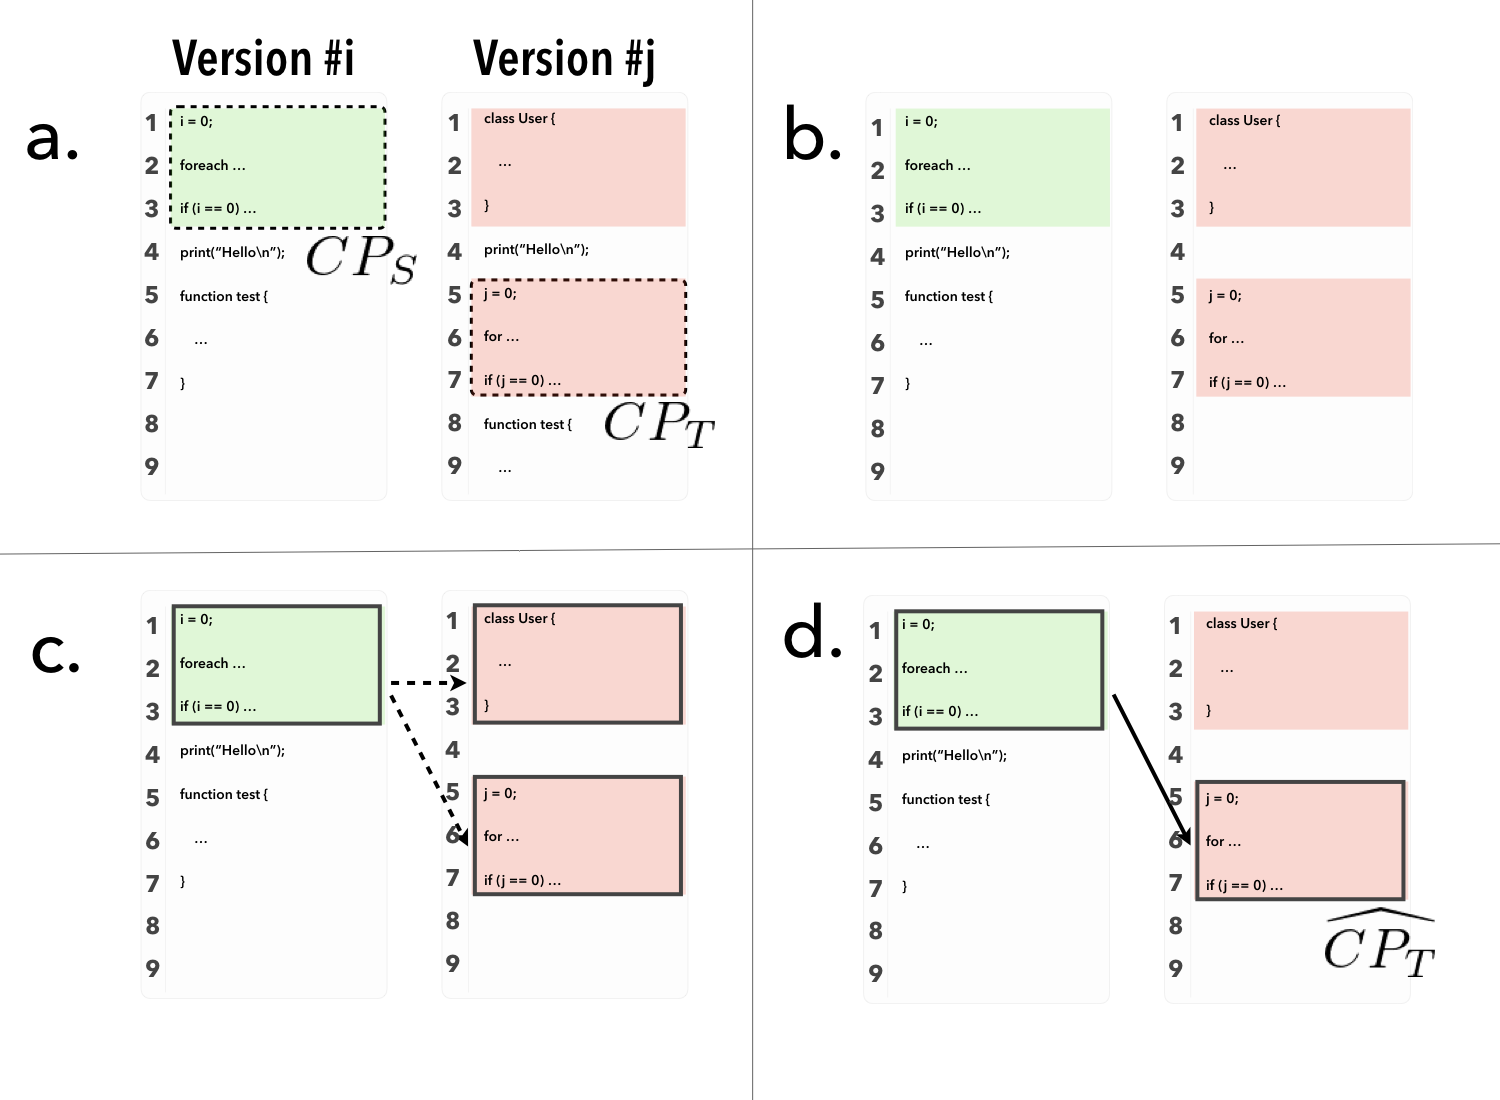
\includegraphics[width=1.0\columnwidth]{algorithm/Cases_003.png}
%       \caption{Case C: $CP_S$ does not include unchanged lines (a) $CP_S$ and $CP_T$ are line 1--3 in the source commit and from line 5--7 in the target commit, respectively. (b) DiffTrack first removes all unchanged lines from the search. (c) It then performs fuzzy string matching on all possible string chunks, and finds the most similar match. (d) DiffTrack finally determines line 5--7 in the target commit as $\widehat{CP_T}$.}~\label{fig:caseC}
%     \vspace{-5mm}
%     \end{figure}



% The two example above demonstrates that unchanged lines in $CP_S$ serve as a useful anchor for determining $\widehat{CP_T}$.
% However, $CP_S$ may not contain any unchanged line as illustrated in Figure \ref{fig:caseC}.
% In this case, DiffTrack first removes all unchanged lines from the search.
% This would result in string chunks (i.e., sets of consecutive code lines) as shown in Figure \ref{fig:caseC}.
% The algorithm then performs fuzzy string matching on all chunks and sub-chunks, and finds the most similar match.

% \subsection{Fuzzy String Matching}
% The DiffTrack algorithm performs fuzzy string matching to identify a code piece most similar to $CP_S$ in the target commit.
% It uses a variant of the Levenshtein distance as a cost function.
% The Levenshtein distance is defined as the minimum number of character operations that are necessary to convert a string to another.
% Character operations include additions, deletions and substitutions.
% In our fuzzy string matching, we calculate the distance on a word basis with different weights on change operations (1, 1, and 2 for additions, deletions and substitutions, respectively).
% For example, the cost of a conversion from ``int x = 1 + 2;'' to ``float x = 1.0;'' is 6 because there are 2 deletions and 2 substitutions.
% Our fuzzy matching also considers the length of $CP_S$ and a possible target code piece ($cp$).
% The DiffTrack algorithm thus uses the following similarity score to find possible a target code piece:

% % \koji{}{Maybe explain why we use word-based similarity rather than char-based?}

% \vspace{-5mm}
% \begin{equation*}
% Sim(cp) = \frac{wp(CP_S) + wp(cp) - LDw(CP_S,\, cp)}{wp(CP_S) + wp(cp)},
% \end{equation*}
% \vspace{-3mm}

% where $wp(x)$ is the word count in text $x$, and $LDw$ is a word-level Levenshtein distance.
% $Sim(cp)$ takes a value between 0 and 1, representing that higher is more similar.
% We use a brute-force approach to find a code piece with the highest similarity score.





\begin{figure}[t]
\centering
  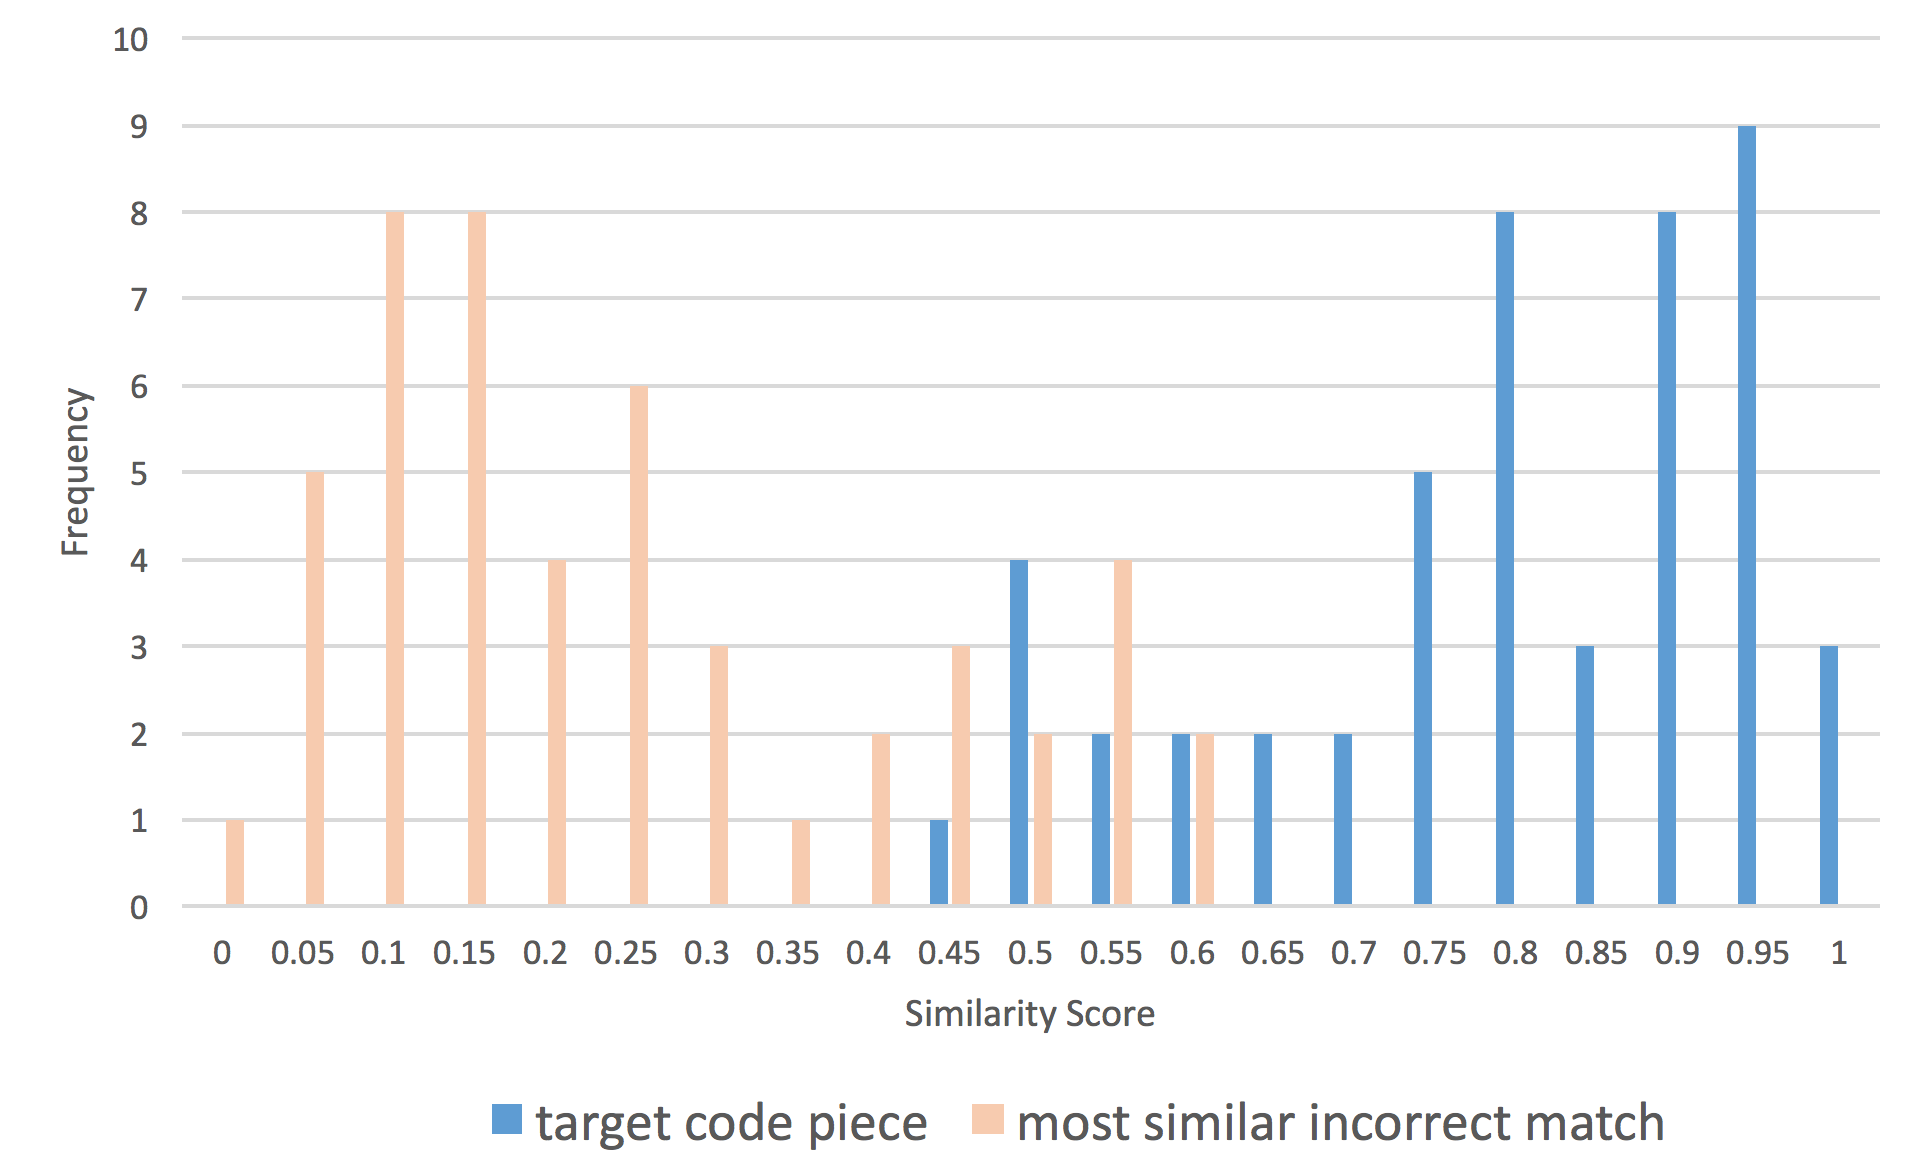
\includegraphics[width=1.0\columnwidth]{algorithm/histogram_sim.png}
  \caption{$CP_T$(青)と$IM$(橙)の文字列的類似度の分布.}~\label{fig:histogram_sim}
\end{figure}









